\section{Thermal Expansion}

\begin{multicols}{2}


\subsection{Explaining Expansion}

\begin{center}
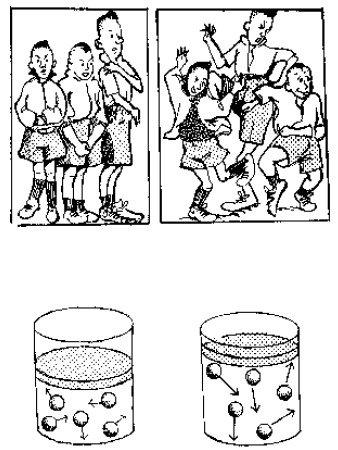
\includegraphics[width=0.4\textwidth]{./img/source/explaining-expansion.png}
\end{center}

\begin{description*}
%\item[Subtopic:]{}
%\item[Materials:]{}
%\item[Setup:]{}
%\item[Procedure:]{}
%\item[Hazards:]{}
%\item[Questions:]{}
%\item[Observations:]{}
\item[Theory:]{}
%\item[Applications:]{}
%\item[Notes:]{}
\end{description*}


\section*{Thermal Expansion of Solids}


\subsection{Ring and Nail}

\begin{center}
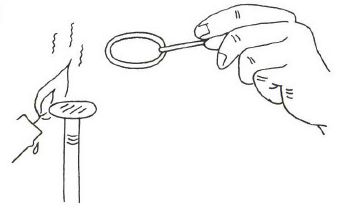
\includegraphics[width=0.4\textwidth]{./img/vso/ring-nail.png}
\end{center}

\begin{description*}
%\item[Subtopic:]{}
\item[Materials:]{}
\item[Setup:]{}
\item[Procedure:]{}
\item[Hazards:]{}
\item[Questions:]{}
\item[Observations:]{}
\item[Theory:]{}
\item[Applications:]{}
\item[Notes:]{}
\end{description*}

\subsection{Expansion of a Coin}

\begin{center}
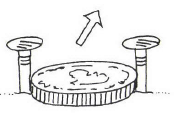
\includegraphics[width=0.3\textwidth]{./img/vso/expansion-coin.png}
\end{center}

\begin{description*}
%\item[Subtopic:]{}
\item[Materials:]{}
\item[Setup:]{}
\item[Procedure:]{}
\item[Hazards:]{}
\item[Questions:]{}
\item[Observations:]{}
\item[Theory:]{}
\item[Applications:]{}
\item[Notes:]{}
\end{description*}

\subsection{Expansion of a Wire}

\begin{center}
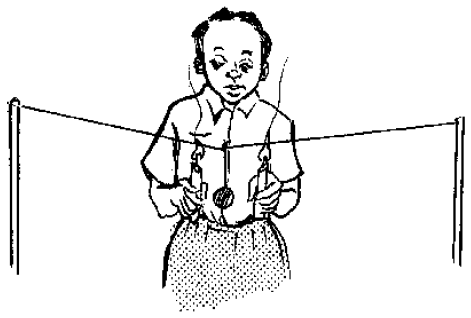
\includegraphics[width=0.4\textwidth]{./img/source/expansion-wire.png}
\end{center}

\begin{description*}
%\item[Subtopic:]{}
\item[Materials:]{}
\item[Setup:]{}
\item[Procedure:]{}
\item[Hazards:]{}
\item[Questions:]{}
\item[Observations:]{}
\item[Theory:]{}
\item[Applications:]{}
\item[Notes:]{}
\end{description*}

\subsection{Breaking Glass}

%\begin{center}
%\includegraphics[width=0.4\textwidth]{./img/source/.png}
%\end{center}

\begin{description*}
%\item[Subtopic:]{}
\item[Materials:]{}
\item[Setup:]{}
\item[Procedure:]{}
\item[Hazards:]{}
\item[Questions:]{}
\item[Observations:]{}
\item[Theory:]{}
\item[Applications:]{}
\item[Notes:]{}
\end{description*}

\subsection{Bimetallic Strip}

\begin{center}
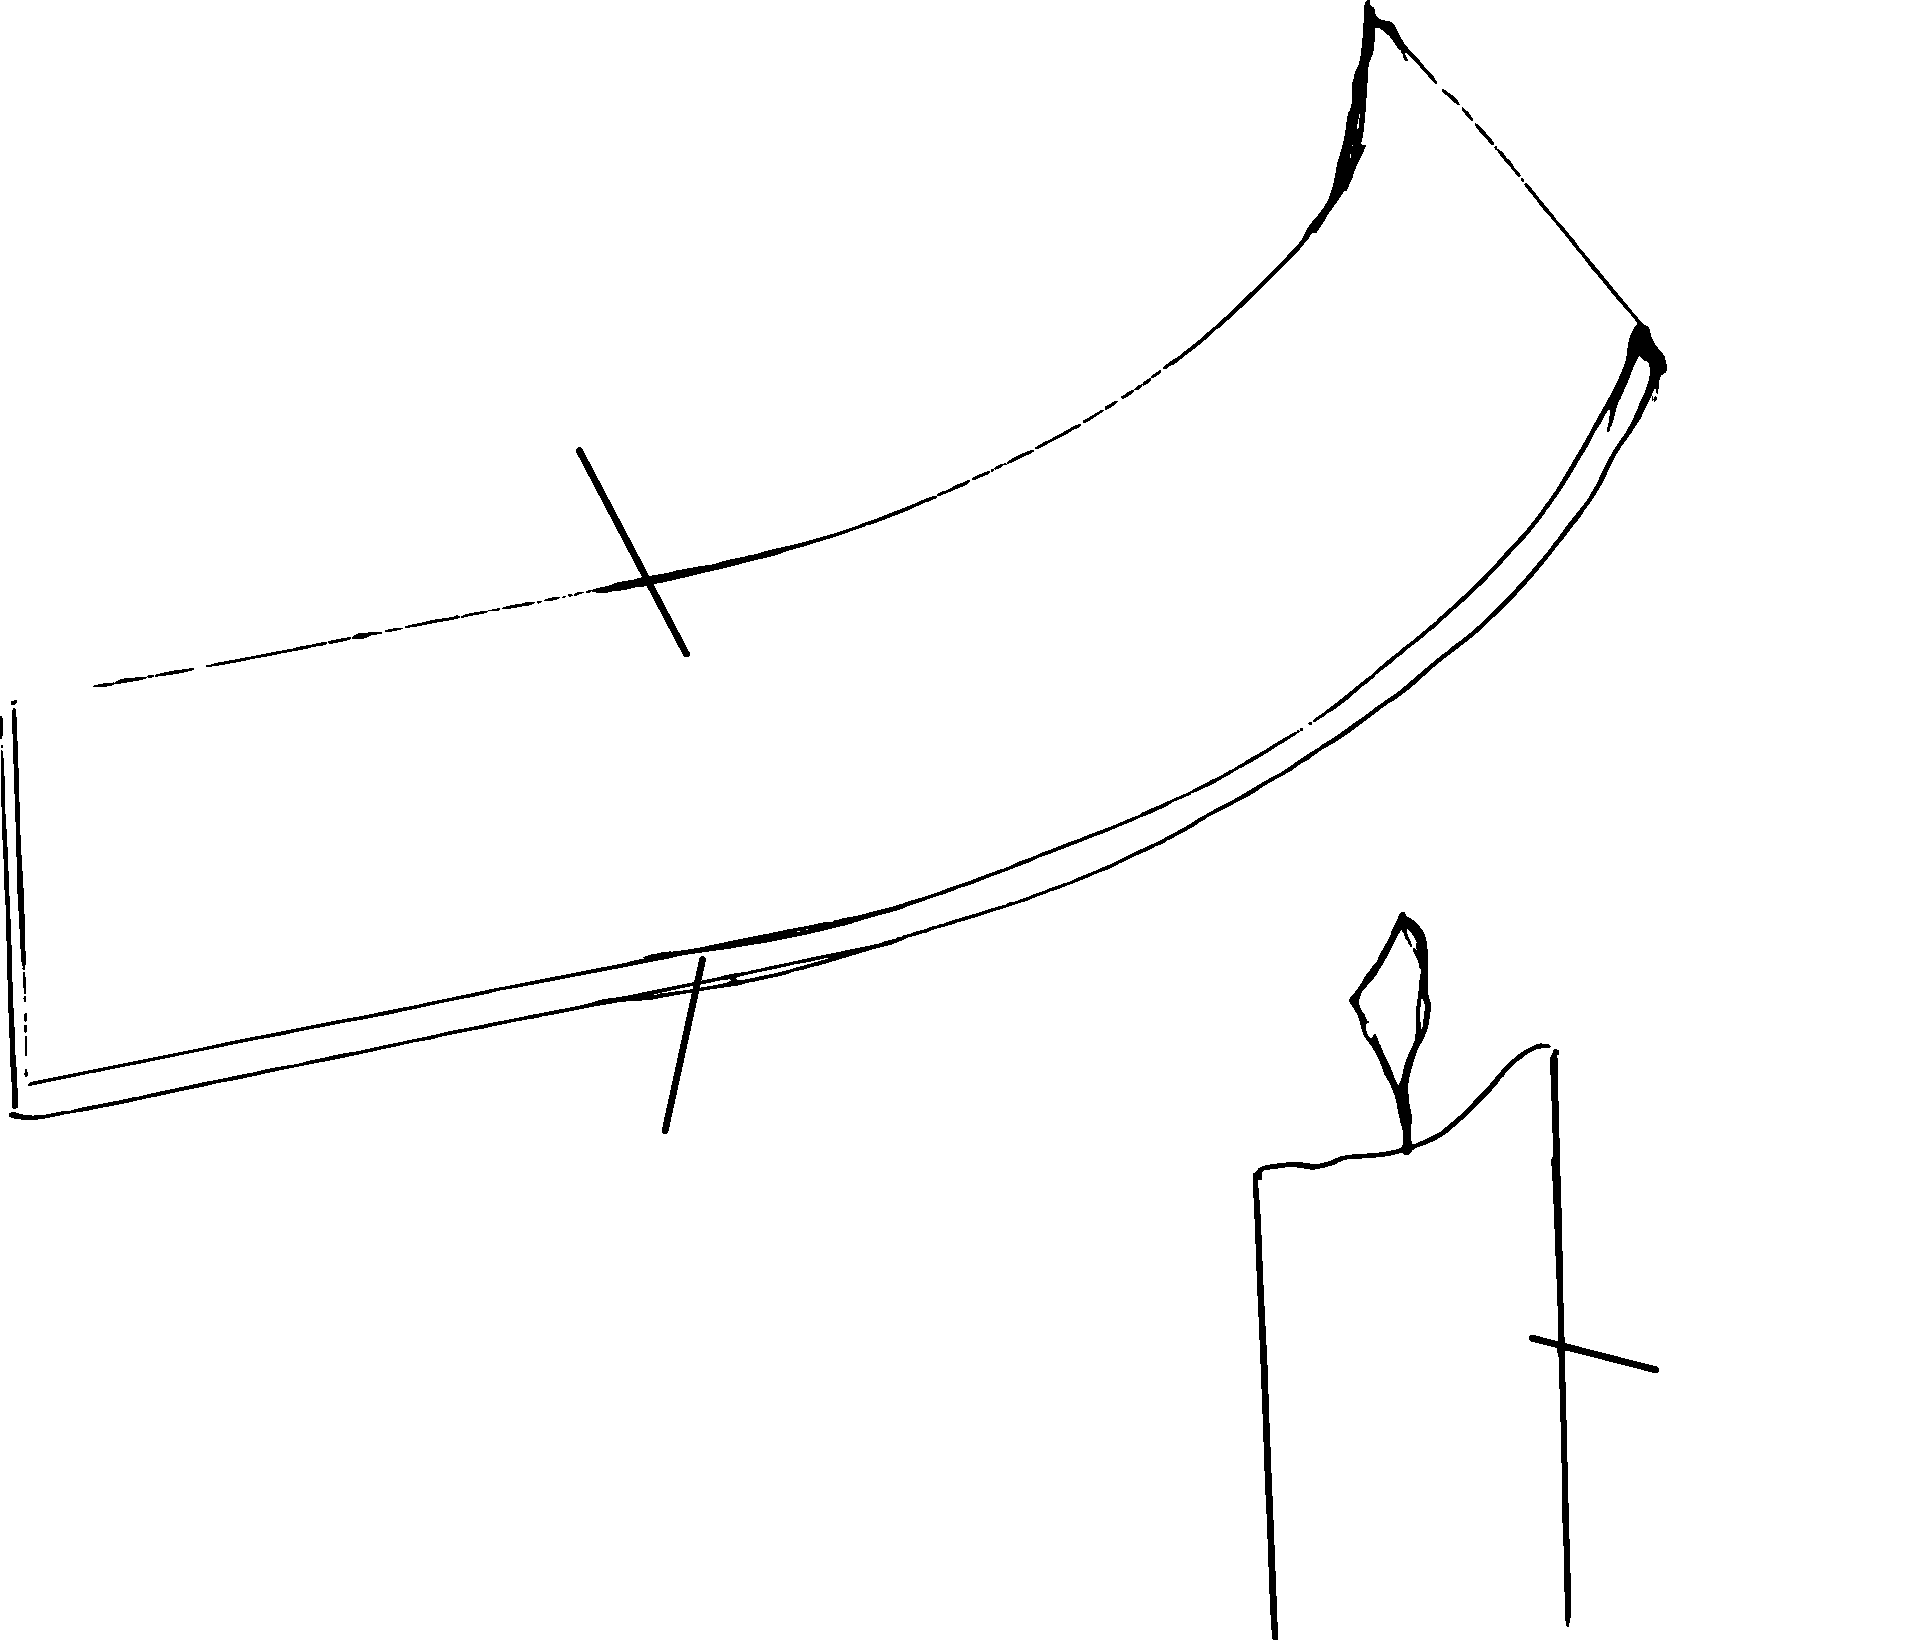
\includegraphics[width=0.4\textwidth]{./img/bimetallic-strip.png}
\end{center}

\begin{description*}
%\item[Subtopic:]{}
\item[Materials:]{}
\item[Setup:]{}
\item[Procedure:]{}
\item[Hazards:]{}
\item[Questions:]{}
\item[Observations:]{}
\item[Theory:]{}
\item[Applications:]{}
\item[Notes:]{}
\end{description*}

\subsection{Thermal Switch}

\begin{center}
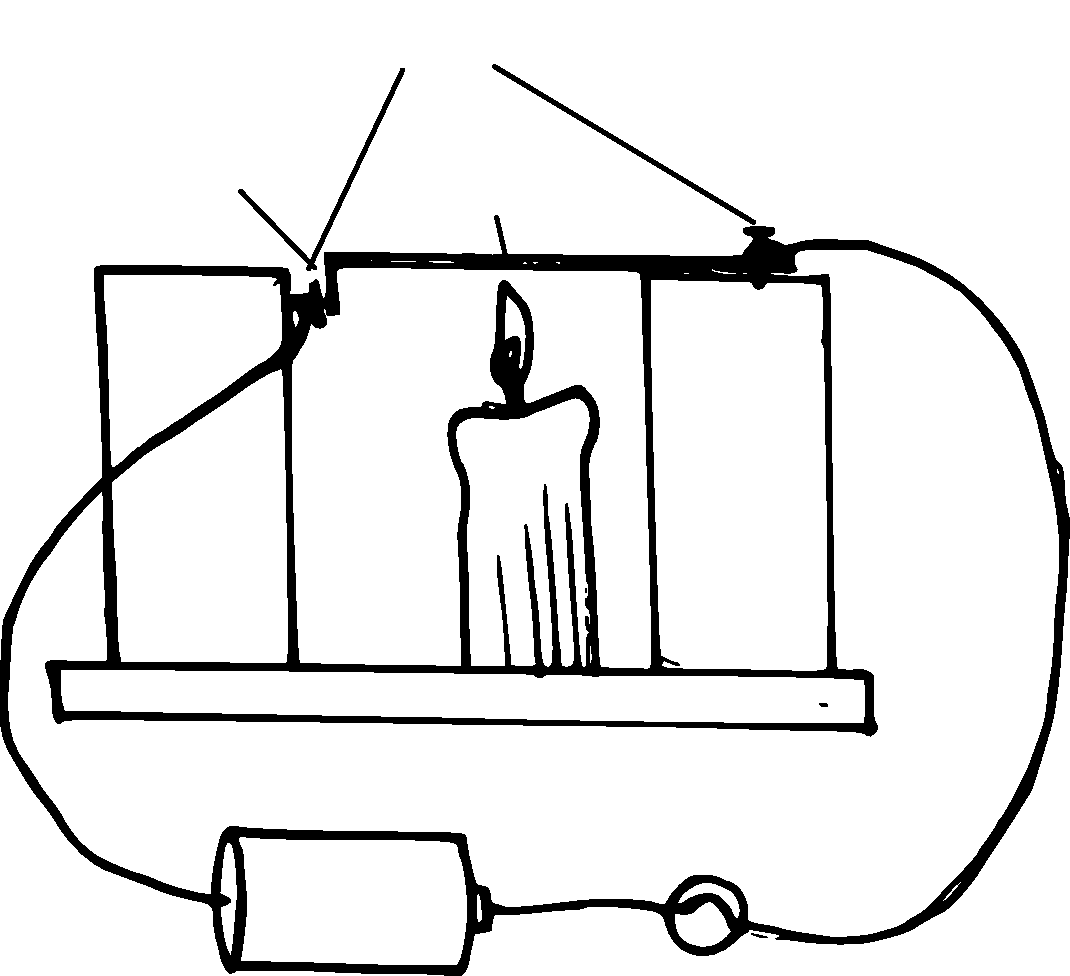
\includegraphics[width=0.4\textwidth]{./img/thermal-switch.png}
\end{center}

\begin{description*}
%\item[Subtopic:]{}
\item[Materials:]{}
\item[Setup:]{}
\item[Procedure:]{}
\item[Hazards:]{}
\item[Questions:]{}
\item[Observations:]{}
\item[Theory:]{}
\item[Applications:]{}
\item[Notes:]{}
\end{description*}

\subsection{Measuring Expansion}

\begin{center}
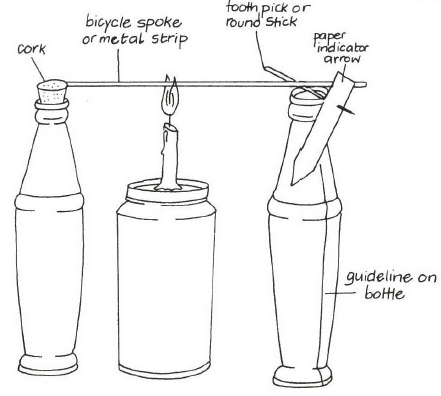
\includegraphics[width=0.4\textwidth]{./img/vso/measuring-expansion.png}
\end{center}

\begin{description*}
%\item[Subtopic:]{}
\item[Materials:]{}
\item[Setup:]{}
\item[Procedure:]{}
\item[Hazards:]{}
\item[Questions:]{}
\item[Observations:]{}
\item[Theory:]{}
\item[Applications:]{}
\item[Notes:]{}
\end{description*}

\subsection{Allowing for Expansion}

\begin{center}
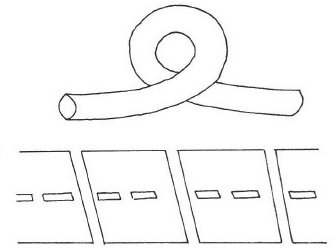
\includegraphics[width=0.4\textwidth]{./img/vso/allowing-expansion.png}
\end{center}

\begin{description*}
%\item[Subtopic:]{}
\item[Materials:]{}
\item[Setup:]{}
\item[Procedure:]{}
\item[Hazards:]{}
\item[Questions:]{}
\item[Observations:]{}
\item[Theory:]{}
\item[Applications:]{}
\item[Notes:]{}
\end{description*}

%==================================================================================================%

\section*{Thermal Expansion of Liquids}


\subsection{Rising Colours}

\begin{center}
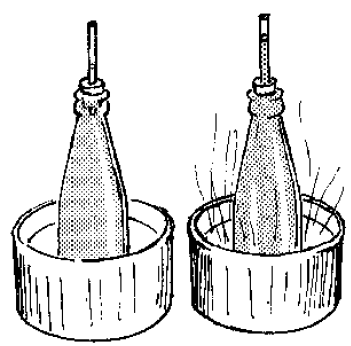
\includegraphics[width=0.4\textwidth]{./img/source/rising-colours.png}
\end{center}

\begin{description*}
%\item[Subtopic:]{}
\item[Materials:]{}
\item[Setup:]{}
\item[Procedure:]{}
\item[Hazards:]{}
\item[Questions:]{}
\item[Observations:]{}
\item[Theory:]{}
\item[Applications:]{}
\item[Notes:]{}
\end{description*}

\subsection{Jumping Coin}

\begin{center}
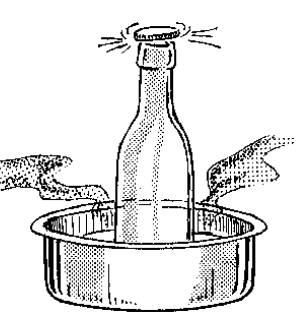
\includegraphics[width=0.4\textwidth]{./img/source/jumping-coin.png}
\end{center}

\begin{description*}
%\item[Subtopic:]{}
\item[Materials:]{}
\item[Setup:]{}
\item[Procedure:]{}
\item[Hazards:]{}
\item[Questions:]{}
\item[Observations:]{}
\item[Theory:]{}
\item[Applications:]{}
\item[Notes:]{}
\end{description*}

\subsection{Liquid Thermometers}

\begin{center}
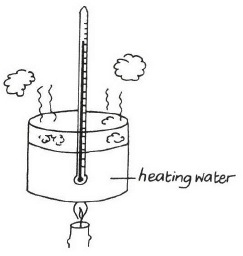
\includegraphics[width=0.4\textwidth]{./img/vso/liquid-thermometers.png}
\end{center}

\begin{description*}
%\item[Subtopic:]{}
\item[Materials:]{}
\item[Setup:]{}
\item[Procedure:]{}
\item[Hazards:]{}
\item[Questions:]{}
\item[Observations:]{}
\item[Theory:]{}
\item[Applications:]{}
\item[Notes:]{}
\end{description*}

\subsection{Allowing for Liquid Expansion}

\begin{center}
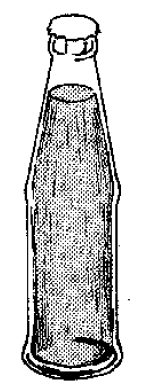
\includegraphics[width=0.2\textwidth]{./img/source/allowing-expansion-liquid.png}
\end{center}

\begin{description*}
%\item[Subtopic:]{}
\item[Materials:]{}
\item[Setup:]{}
\item[Procedure:]{}
\item[Hazards:]{}
\item[Questions:]{}
\item[Observations:]{}
\item[Theory:]{}
\item[Applications:]{}
\item[Notes:]{}
\end{description*}

%==================================================================================================%

\section*{Thermal Expansion of Gases}
\textbf{Charles' Law} states that \\
\textbf{Boyle's Law} state that 

% Charles' Law

\subsection{Bottle Crush}

\begin{center}
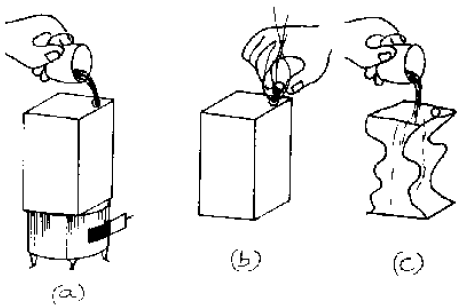
\includegraphics[width=0.4\textwidth]{./img/source/bottle-crush.png}
\end{center}

\begin{description*}
%\item[Subtopic:]{}
\item[Materials:]{Plastic water bottle, boiling water, cold water}
%\item[Setup:]{}
\item[Procedure:]{Pour some boiling water into the bottle and cap it immediately. Shake it to make sure all the air inside is heated. Pour out the hot water and cap the bottle. Then pour cold water on the outside of the bottle.}
%\item[Hazards:]{}
%\item[Questions:]{}
\item[Observations:]{Upon pouring the cold water, the bottle crushes.}
\item[Theory:]{Boiling water is used initially to increase the temperature of the air in the bottle. It is removed and the bottle is sealed, forcing the pressure to remain constant. As the air inside the bottle cools, it decreases the volume, causing the bottle to be crushed from the inside. $T \propto V$ when $P$ is constant.}
\item[Applications:]{Atmospheric pressure}
%\item[Notes:]{This is an application of Charles' Law. For more, see \nameref{}.}
\end{description*}

\subsection{Egg Suck}

\begin{center}
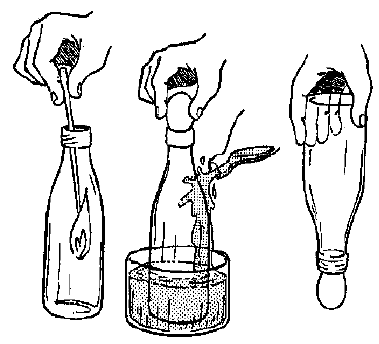
\includegraphics[width=0.4\textwidth]{./img/source/egg-suck.png}
\end{center}

\begin{description*}
%\item[Subtopic:]{}
\item[Materials:]{}
\item[Setup:]{}
\item[Procedure:]{}
\item[Hazards:]{}
\item[Questions:]{}
\item[Observations:]{}
\item[Theory:]{}
\item[Applications:]{}
\item[Notes:]{}
\end{description*}

\subsection{Spray Balloon}

%\begin{center}
%\includegraphics[width=0.4\textwidth]{./img/source/.png}
%\end{center}

\begin{description*}
%\item[Subtopic:]{}
\item[Materials:]{}
\item[Setup:]{}
\item[Procedure:]{}
\item[Hazards:]{}
\item[Questions:]{}
\item[Observations:]{}
\item[Theory:]{}
\item[Applications:]{}
\item[Notes:]{}
\end{description*}

% Boyle's Law

\subsection{Syringe Suck}

%\begin{center}
%\includegraphics[width=0.4\textwidth]{./img/source/.png}
%\end{center}

\begin{description*}
%\item[Subtopic:]{}
\item[Materials:]{}
\item[Setup:]{}
\item[Procedure:]{}
\item[Hazards:]{}
\item[Questions:]{}
\item[Observations:]{}
\item[Theory:]{}
\item[Applications:]{}
\item[Notes:]{}
\end{description*}

\subsection{Balloon Blow}

%\begin{center}
%\includegraphics[width=0.4\textwidth]{./img/source/.png}
%\end{center}

\begin{description*}
%\item[Subtopic:]{}
\item[Materials:]{}
\item[Setup:]{}
\item[Procedure:]{}
\item[Hazards:]{}
\item[Questions:]{}
\item[Observations:]{}
\item[Theory:]{}
\item[Applications:]{}
\item[Notes:]{}
\end{description*}

\subsection{Balloon Suck}

%\begin{center}
%\includegraphics[width=0.4\textwidth]{./img/source/.png}
%\end{center}

\begin{description*}
%\item[Subtopic:]{}
\item[Materials:]{}
\item[Setup:]{}
\item[Procedure:]{}
\item[Hazards:]{}
\item[Questions:]{}
\item[Observations:]{}
\item[Theory:]{}
\item[Applications:]{}
\item[Notes:]{}
\end{description*}

%==================================================================================================%


\end{multicols}

\pagebreak